\begin{section}{Introduction to Induction}

Consider the claims:
\begin{enumerate}[label=\textrm{(\alph*)}]
\item For all $n\in\mathbb{N}$, $\displaystyle 1+2+3+\cdots +n=\frac{n(n+1)}{2}$.
\item For all $n\in\mathbb{N}$, $n^{2}+n+41$ is prime.
\end{enumerate}
Let's take a look at potential proofs.

\bigskip

\noindent \emph{``Proof'' of (a).} If $n=1$, then $1=\frac{1(1+1)}{2}$.  If $n=2$, then $1+2=3=\frac{2(2+1)}{2}$.  If $n=3$, then $1+2+3=6=\frac{3(3+1)}{2}$, and so on. \hfill \qed

\bigskip

\noindent \emph{``Proof'' of (b).} If $n=1$, then $n^{2}+n+41=43$, which is prime.  If $n=2$, then $n^{2}+n+41=47$, which is prime.  If $n=3$, then $n^{2}+n+41=53$, which is prime, and so on. \hfill \qed

\bigskip

Are these actual proofs?  \textbf{NO!}  In fact, the second claim isn't even true.  If $n=41$, then $n^{2}+n+41=41^{2}+41+41=41(41+1+1)$, which is not prime since it has 41 as a factor.  It turns out that the first claim is true, but what we wrote cannot be a proof since the same type of reasoning when applied to the second claim seems to prove something that isn't actually true.  We need a rigorous way of capturing ``and so on'' and a way to verify whether it really is ``and so on.''

\begin{axiom}[Axiom of Induction]\label{axiom:induction}
Let $S\subseteq \mathbb{N}$ such that both
\begin{enumerate}[label=\textrm{(\roman*)}]
\item $1\in S$, and
\item if $k\in S$, then $k+1\in S$.
\end{enumerate}
Then $S=\mathbb{N}$.
\end{axiom}

Recall that an axiom is a basic mathematical assumption.  That is, we are assuming that the Axiom of Induction is true, which I'm hoping that you can agree is a pretty reasonable assumption.  We can think of the first hypothesis as saying that we have a first rung of a ladder.  The second hypothesis says that if we have any arbitrary rung of the ladder, then we can always get to the next rung.  Taken together, this says that we can get from the first rung to the second, from the second to the third, and in general, from any $k$th rung to the $(k+1)$st rung.

\begin{theorem}[Principle of Mathematical Induction]\label{thm:PMI}
Let $P(1), P(2), P(3), \ldots$ be a sequence of statements, one for each natural number.\footnote{Think of $P(n)$ as a predicate, where $P(1)$ is the statement that corresponds to substituting in the value 1 for $n$.} Assume
\begin{enumerate}[label=\textrm{(\roman*)}]
\item $P(1)$ is true, and
\item if $P(k)$ is true, then $P(k+1)$ is true.
\end{enumerate}
Then $P(n)$ is true for all $n\in\mathbb{N}$.\footnote{\emph{Hint:} Let $S=\{k\in \mathbb{N}\mid P(k) \text{ is true}\}$ and use the Axiom of Induction.  The set $S$ is sometimes called the \textbf{truth set}.  Your job is to show that the truth set is all of $\mathbb{N}$.}
\end{theorem}

The Principal of Mathematical Induction (PMI) provides us with a process for proving statements of the form: ``For all $n\in\mathbb{N}$, $P(n)$,'' where $P(n)$ is some predicate involving $n$.  Hypothesis (i) above is called the \textbf{base step} while (ii) is called the \textbf{inductive step}.

You should not confuse \emph{mathematical induction} with \emph{inductive reasoning} associated with the natural sciences. Inductive reasoning is a scientific method whereby one induces general principles from observations. On the other hand, mathematical induction is a deductive form of reasoning used to establish the validity of a proposition.

\begin{skeleton}[Proof of $(\forall n\in\mathbb{N})P(n)$ by Induction]
Here is the general structure for a proof by induction.

\begin{center}
\framebox{
\begin{minipage}{6in}
\vspace{.1in}
\begin{proof}
We proceed by induction.
\begin{enumerate}\setlength{\itemsep}{0in}
\item[(i)] Base step: \emph{[Verify that $P(1)$ is true. This often, but not always, amounts to plugging $n=1$ into two sides of some claimed equation and \underline{verifying} that both sides are actually equal.]}

\item[(ii)] Inductive step:  \emph{[Your goal is to prove ``For all $k\in\mathbb{N}$, if $P(k)$ is true, then $P(k+1)$ is true.'']} Let $k\in\mathbb{N}$ and assume that $P(k)$ is true. \emph{[Do something to derive that $P(k+1)$ is true.]} Therefore, $P(k+1)$ is true.
\end{enumerate}
Thus, by the PMI, $P(n)$ is true for all $n\in\mathbb{N}$.
\end{proof}
\end{minipage}
}
\end{center}
\end{skeleton}

Prove the next few theorems using induction.

\begin{theorem}
For all $n\in\mathbb{N}$, $\displaystyle \sum_{i=1}^{n}i=\frac{n(n+1)}{2}$.\footnote{Recall that $\displaystyle \sum_{i=1}^{n}i=1+2+3+\cdots +n$, by definition.  Also, this theorem should look familiar from calculus.}
\end{theorem}

\begin{theorem}
For all $n\in\mathbb{N}$, 3 divides $4^{n}-1$.
\end{theorem}

\begin{theorem}
For all $n\in\mathbb{N}$, 6 divides $n^{3}-n$.
\end{theorem}

\begin{theorem}
Let $p_{1}, p_{2}, \ldots, p_{n}$ be $n$ distinct points arranged on a circle.  Then the number of line segments joining all pairs of points is $\frac{n^{2}-n}{2}$.
\end{theorem}

\begin{problem}
A special chessboard is $2$ squares wide and $n$ squares long.  Using $n$ dominoes that are $1$ square by $2$ squares, there are many ways to perfectly cover this chessboard with no overlap.  How many?  Prove your answer.
\end{problem}

\begin{problem}\label{prob:L-shapes}
Another chessboard is $2^n$ squares wide and $2^n$ squares long.  However, one of the squares has been cut out, but you don't know which one!  You have a bunch of L-shapes made up of $3$ squares.  Prove that you can perfectly cover this chessboard with the L-shapes (with no overlap) for any $n\in\mathbb{N}$. Figure~\ref{fig:L-shapes} depicts one possible covering for the case involving $n=2$.
\end{problem}

\begin{figure}[ht]
\begin{center}
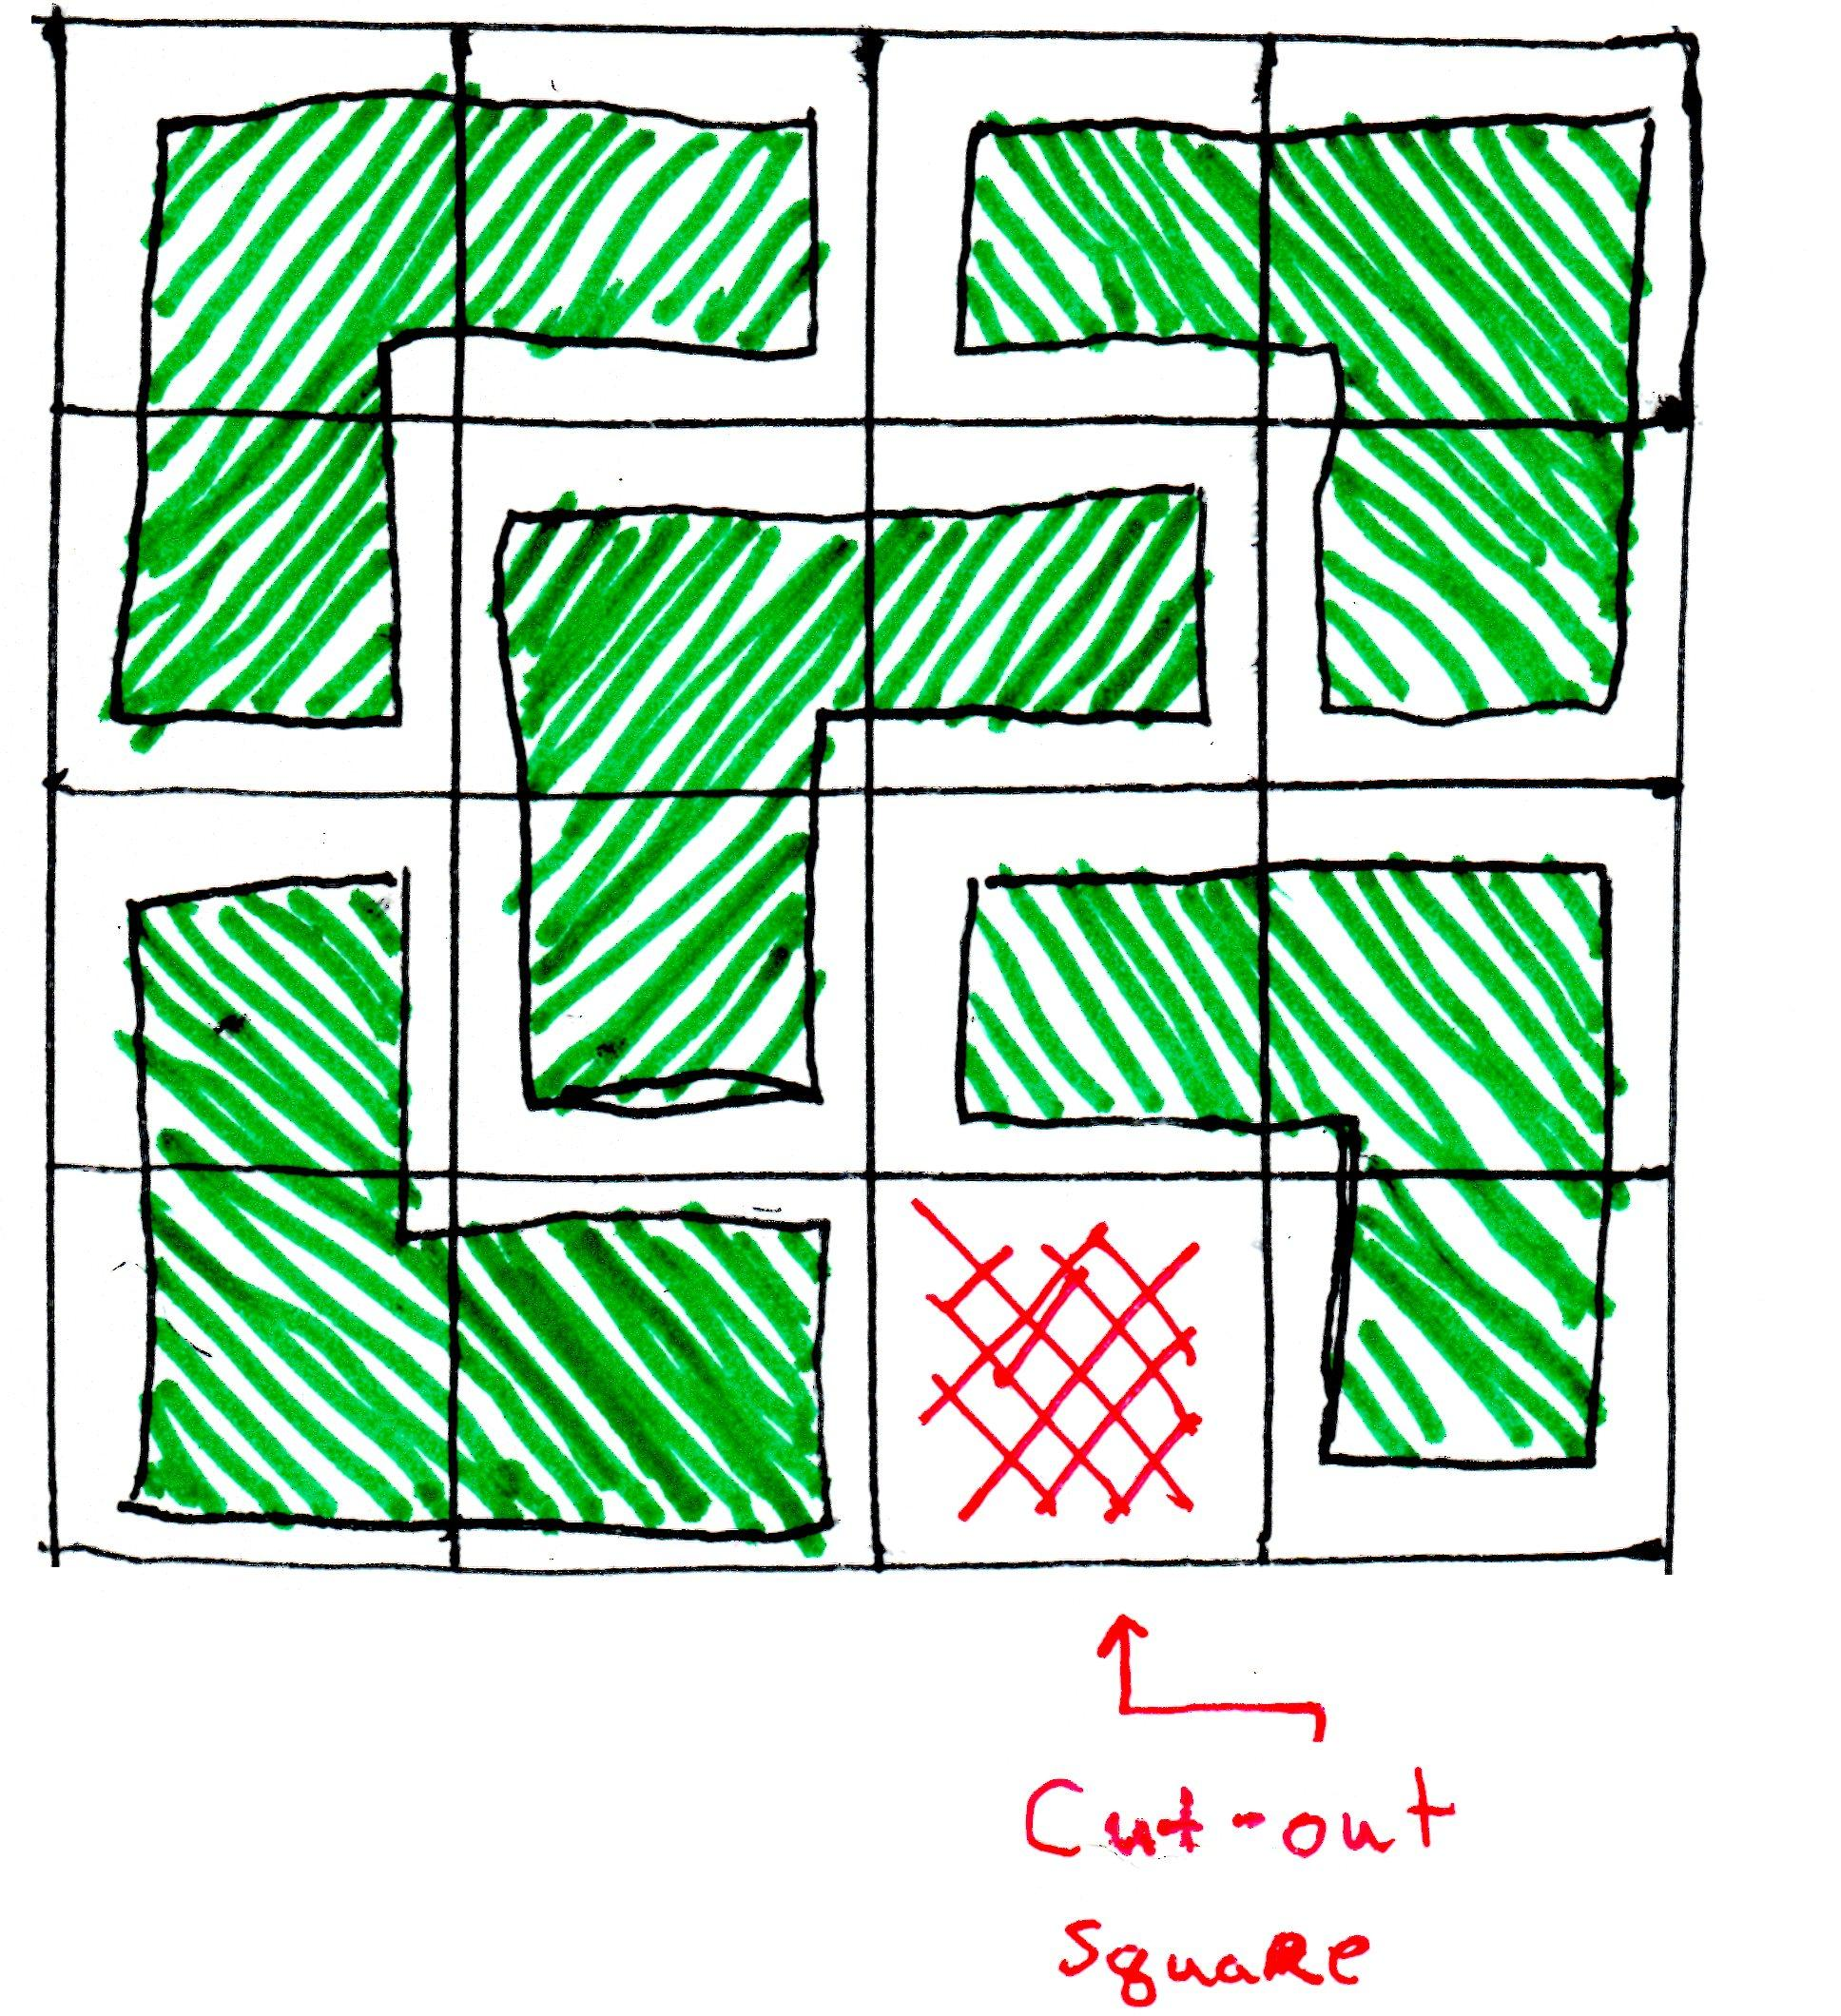
\includegraphics[width=2in]{L-shapes.jpg}
\end{center}
\vspace{-.5cm}
\caption{One possible covering for the case involving $n=2$ for Problem~\ref{prob:L-shapes}.}
\label{fig:L-shapes}
\end{figure}

\end{section}